\documentclass[12pt]{article}
\usepackage{amsmath,float,booktabs,rotating,graphicx,csquotes}
\usepackage[a4paper,top=2cm,bottom=2cm,left=3cm,right=3cm,marginparwidth=1.75cm]{geometry}
\usepackage[english]{babel}
\usepackage[onehalfspacing]{setspace} % Sets line spacing to 1.5
\usepackage[colorlinks=true, allcolors=blue]{hyperref}
\usepackage[ruled] {algorithm2e}
\graphicspath{ {./images/} }  % Look within the "images" folder for Images. 

\newcommand{\latex}{\LaTeX\ }
\renewcommand*\familydefault{\sfdefault}

\begin{document}
\begin{center}
    \vspace{0.8cm}
    \Large
    \textbf{Short Guide to Working with an Overleaf Project}
    
    \vspace{0.5cm}
    
    Dr. Daniel C. Doolan\\
    \large
    \today
\end{center}
\singlespacing
\tableofcontents  % Display Table of Contents
\listoffigures    % Display List of Figures
\clearpage
\onehalfspacing
% The main body / content of the report begins here.

\section{Create an Overleaf Account}
Go to (\url{https://www.overleaf.com}) and register for a new account by supplying an ``email addresss'' and ``password''. Once an account has been created check your email, as you will receive an automated email with a link to verify the registration process.

\section{Join a Read Only Project from a Link}
Upon selection of a Link to a Read-only Overleaf Project, you will be presented with an ``invite to join'' screen (Figure~\ref{fig:00:OverleafInviteToJoin}). Clicking the ``Join Project'' button will provide you with access to the project. 

\begin{figure}[H]
\begin{center}

\includegraphics[width=.70\linewidth]{00-InviteToJoinProject.png}
\caption{Invite to Join an Overleaf Project} \label{fig:00:OverleafInviteToJoin}
\end{center}
\end{figure}

\section{Loaded Overleaf Project User Interface}
Upon loading of an Overleaf Project provided as a Read-only link, the Overleaf editor will be presented, with panels for the File Structure, Document Outline, the Source Code Editor and the Rendered view of the Output document, as depicted in Figure~\ref{fig:04:OverleafInterface}.

\begin{figure}[H]
\begin{center}
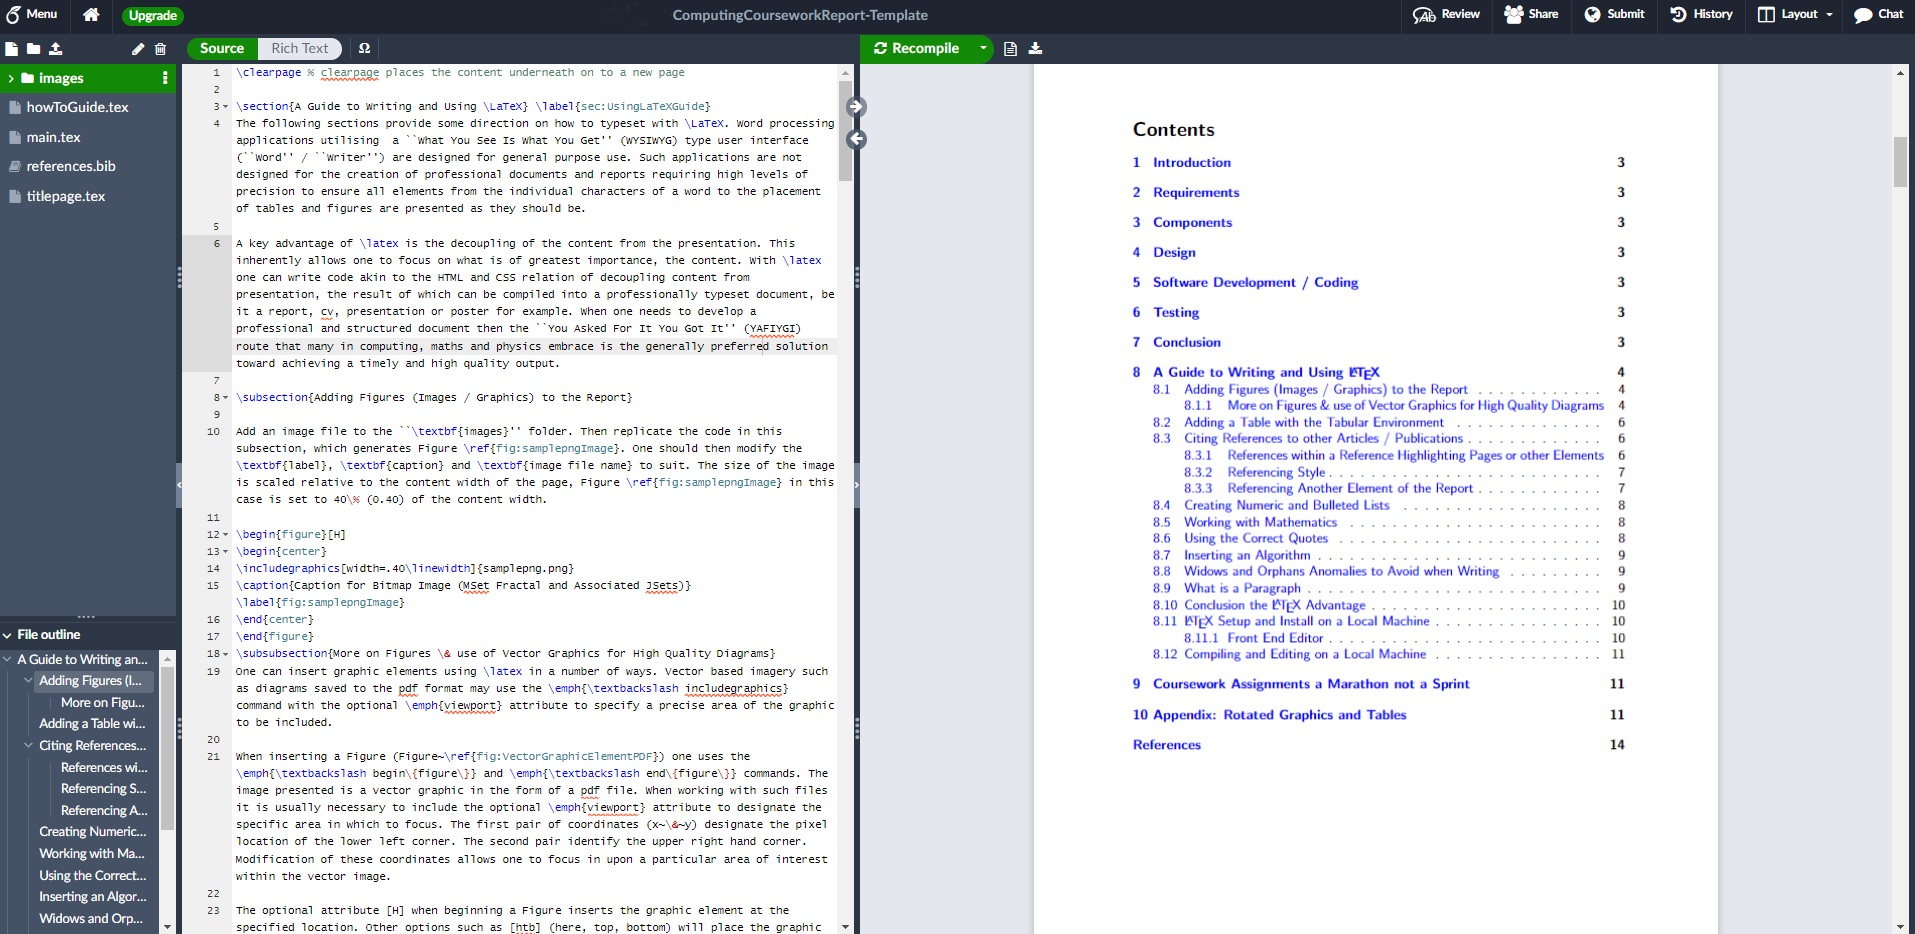
\includegraphics[width=.85\linewidth]{04-overleaf-NewProject.png}
\caption{Overleaf Project Main User Interface Screen} \label{fig:04:OverleafInterface}
\end{center}
\end{figure}

\clearpage
\section{Creating a new Editable Project}
Select the Overleaf ``Menu'' located in the top left of the Editor (Figure~\ref{fig:05:OverleafMenu}).

\begin{figure}[H]
\begin{center}

\includegraphics[width=.35\linewidth]{05-navigateToHome-ProjectsScreen.png}
\caption{Overleaf Menu} \label{fig:05:OverleafMenu}
\end{center}
\end{figure}

Select the ``Copy Project'' option from the resulting screen (Figure~\ref{fig:08:MenuOptions}).

\begin{figure}[H]
\begin{center}
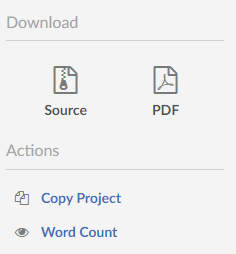
\includegraphics[width=.35\linewidth]{08-FromMenu-GetWordCount.png}
\caption{Overleaf Menu Options} \label{fig:08:MenuOptions}
\end{center}
\end{figure}

Then enter a ``New Name'' for the Project in the ``Copy Project'' dialogue (Figure~\ref{fig:10:CopyProjectDialogue}).

\begin{figure}[H]
\begin{center}
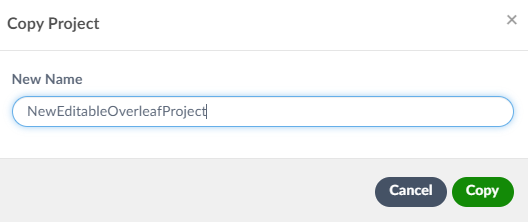
\includegraphics[width=.75\linewidth]{10-CopyProject-Rename.png}
\caption{Copy Project Dialogue} \label{fig:10:CopyProjectDialogue}
\end{center}
\end{figure}

\clearpage
\section{Creating a new Project from a Zip file}
From the ``Home'' or ``Project'' screen (\url{https://www.overleaf.com/project}) presented in Figure~\ref{fig:11:ProjectScreenMenu}, one can select ``New Project'' providing a selection of options. Choose the ``Upload Project'' option (Figure~\ref{fig:06:NewProject}) to upload a ``{\tt .zip}'' file of a project from your local machine. Such Overleaf Project ``{\tt .zip}'' files could be found on GitHub for example. One can also download an Overleaf Source file (`{\tt .zip}''), by clicking on the ``Source'' option of an existing project as seen in Figure~\ref{fig:08:MenuOptions}.

\begin{figure}[H]
\begin{minipage}[t]{7.4cm}
\begin{center}
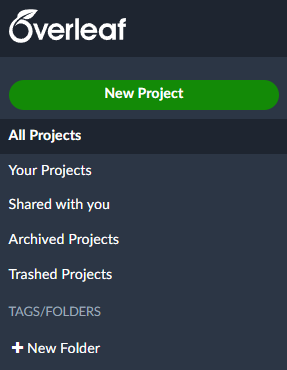
\includegraphics[width=.5\linewidth]{11-ProjectScreenMenu.png}
\caption{Overleaf Project Screen}
\label{fig:11:ProjectScreenMenu}
\end{center}
\end{minipage}
\hfill
\begin{minipage}[t]{7.4cm}
\begin{center}
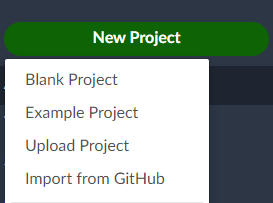
\includegraphics[width=.5\linewidth]{06-NewProject.png}
\caption{New Project $>$ Upload Project}
\label{fig:06:NewProject}
\end{center}
\end{minipage}
\end{figure}

\section{Assessing Document Word Count}
One can access the document word count via the Overleaf Menu in the upper left corner of the UI (Figure~\ref{fig:05:OverleafMenu}). The resulting menu (Figure~\ref{fig:08:MenuOptions}) provides the option of ``Word Count''. Selecting the ``Word Count'' option will yield a dialogue such as that depicted in Figure~\ref{fig:09:WordCount}. It provides an assessment of the word count, number of headings, and the volume of maths included in the document.  

\begin{figure}[H]
\begin{center}
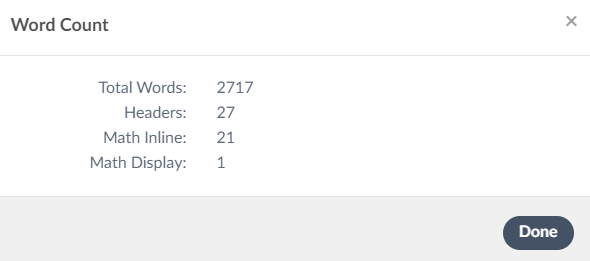
\includegraphics[width=.55\linewidth]{09-GetWordCountOutput.png}
\caption{Word Count Dialogue} \label{fig:09:WordCount}
\end{center}
\end{figure}

\section{Conclusion}
Overleaf is a useful online tool help you create professional written reports, without the need of having to install the likes of MikTeX on your local system along with a separate front end editor. This guide highlights a few of the ways one can get up and running. 
\end{document}